\section{Introduction}
In autonomous driving, scenes primarily consist of two types of entities: dynamic and stationary. Dynamic entities encompass objects capable of movement and interaction, such as vehicles (cars, bicycles, motorcycles, trucks), and pedestrians. Stationary entities, on the other hand, are immobile objects and abstract structures such as lane markings, crosswalks, road signs, traffic lights, barriers, and road surfaces, that regulate traffic and ensure the safe and orderly movement of dynamic entities. Furthermore, abstract stationary entities -such as lanes and centerlines- are defined in relation to other stationary objects or specific rules of the driving environment.

For a fully autonomous driving system, it is essential not only to detect stationary entities but also to understand their interrelationships. The challenge of identifying and understanding these connections between stationary objects is referred to as the \textit{road topology} problem. For instance, multiple lanes may converge into one or a few, or a single lane may split into several. This complexity increases at intersections, where numerous lanes interact. Additionally, some traffic lights control only specific lanes. Accurately localizing, categorizing, and understanding the relationships between stationary entities are essential for downstream tasks such as planning and control in autonomous driving systems.

An alternative solution to this problem is the utilization of High-Definition Maps (HDMaps), which provide pre-computed maps of stationary entities. However, HDMaps are expensive to produce, cover only limited geographic areas, and cannot reflect recent changes on the road, requiring continuous updates. Furthermore, errors introduced by the Global Navigation Satellite System (GNSS) receiver on the vehicle can lead to localization inaccuracies. These inaccuracies may cause discrepancies between the actual position of the vehicle and the HDMap data, potentially resulting in drifts in the map-based guidance system. In response to these challenges, automatic HDMap construction has gained significant attention in recent years for two primary reasons \cite{li2022hdmapnet, liu2023vectormapnet, liao2022maptr, can2021structured}. First, it can reduce reliance on HDMaps for autonomous driving. Second, it lowers the cost of creating and maintaining HDMaps, thereby minimizing the need for human effort.

% The introduction of the OpenLane-V2 dataset \cite{wang2024openlane} marks a significant milestone in research on multi-camera road topology problems. This dataset includes annotations for centerlines and traffic elements and, crucially, provides centerline labels even in intersection areas where lane markings are absent. It facilitates the development of multi-camera-based solutions (3D, Bird’s Eye View (BEV), Perspective View (PV)) for comprehensive scene understanding, including complex road connections and scenarios where road lines are missing. Notably, the dataset adopts the \textit{centerline} concept to represent lanes and expands upon it with the \textit{lane segment} concept. It provides detailed information on the relationships among lane centerlines (or lane segments) and between lane centerlines and traffic elements (such as traffic lights and traffic signs) across various road configurations.

\begin{figure}[tb]
  \centering
  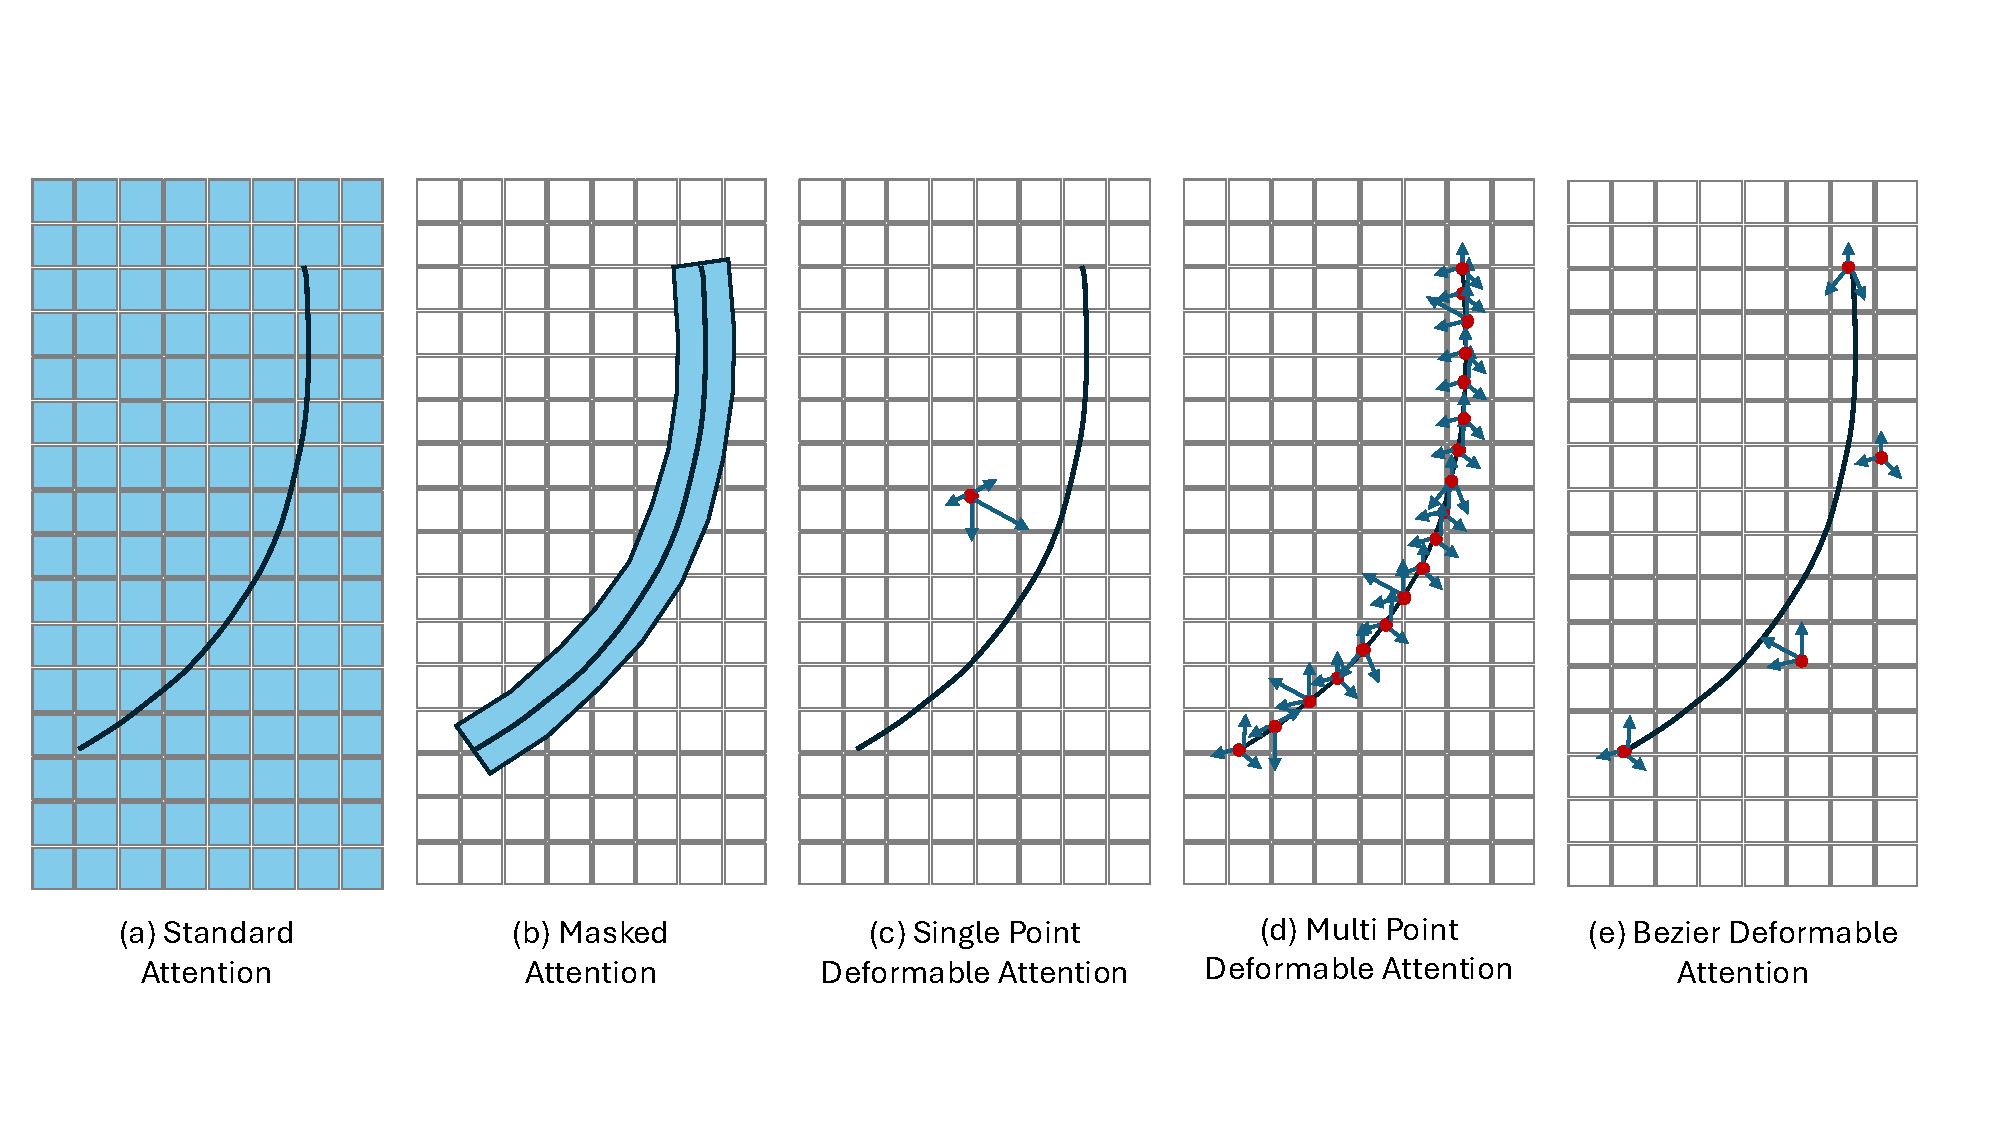
\includegraphics[width=\linewidth]{attention_types.pdf}
  \caption{Comparison of various cross-attention mechanisms within the decoder architecture for polyline structures.}
  \label{fig: attention_types}
\end{figure}

In the context of polyline structures, such as centerlines and lane dividers, the application of standard cross attention \cite{can2021structured, liu2023petrv2}, deformable cross attention \cite{li2023graph, wu2023topomlp, liao2022maptr, luo2023latr, li2023lanesegnet, liu2023vectormapnet, bai2023curveformer, zhou2024himap, choi2024mask2map, liu2024leveraging, xu2024insmapper, yu2023scalablemap}, and masked cross attention \cite{qiao2023end, ding2023pivotnet, zhou2024himap, kalfaoglu2024topomaskv2} is common. Masked attention \cite{cheng2022masked}, as illustrated in Figure \ref{fig: attention_types}b, requires tuning hyperparameters for polyline width and uses a thresholding mechanism to differentiate between foreground and background. Moreover, to prevent the failure of the attention mechanism, a foreground check is performed for every query, increasing complexity and reducing deployment efficiency. In contrast, deformable attention \cite{zhudeformable} can be implemented in two primary ways. The first, Single-Point Deformable Attention (SPDA), shown in Figure \ref{fig: attention_types}c, limits attention for each polyline instance to a single point, typically a learnable query embedding or the center point of the polyline’s bounding box \cite{liu2023vectormapnet, li2023graph, wu2023topomlp}. However, this method restricts attention to a local scope, making it unsuitable for elongated, thin polyline structures.

The second method for implementing deformable attention, Multi-Point Deformable Attention (MPDA), as shown in Figure \ref{fig: attention_types}d, involves distributing attention around every predicted dense lane point \cite{liao2022maptr, yuan2024streammapnet, luo2023latr, xu2024insmapper, chen2025maptracker}. From the MPDA perspective, there are two primary approaches: point query-based methods and instance query-based methods. Point query-based methods are inherently complex because each query represents a single point, and increasing the number of points per instance proportionally increases the complexity \cite{liao2022maptr, liao2024maptrv2, luo2023latr, ding2023pivotnet, li2024enhancing}. Conversely, instance query-based methods are more efficient \cite{li2023lanesegnet, yuan2024streammapnet}. However, a gap in the literature exists, as instance query methods utilizing Bezier control points \cite{wu2023topomlp, li2023graph} have not applied MPDA, relying instead on SPDA.

This study focuses on enhancing centerline detection performance within the broader context of road topology understanding. First, the integration of MPDA into Bezier keypoint-dependent transformer decoder structures is introduced. This adaptation is considered crucial because, unlike other dense polyline prediction methods, the Bezier representation \cite{li2023lanesegnet} \cite{yuan2024streammapnet}, leverages its inherently compact nature to improve the computational efficiency of polyline prediction. By incorporating MPDA into the Bezier keypoint-dependent transformer decoder, the method can more effectively handle elongated and thin polyline structures.

To further optimize the balance between performance and computational complexity, Bezier Deformable Attention (BDA) is introduced. As illustrated in Figure \ref{fig: attention_types}e, this method generates deformable attention around predicted Bezier points for centerline prediction. BDA significantly outperforms SPDA while maintaining a negligible performance difference. The improvement, as well as the reason for not observing an increase in computational complexity, is attributed to the use of control points across different attention heads, rather than relying on a single point to drive all attention heads. Additionally, SPDA requires learning an additional regression target for the center of the bounding box of the centerline. Furthermore, BDA achieves slightly better performance than the MPDA adaptation to the Bezier concept, with slightly less computational overhead. Unlike MPDA, BDA eliminates the need to convert Bezier keypoints into multiple polyline points within each transformer decoder layer, thereby reducing computational complexity. %Our method, designated as Topology with Bezier Deformable Attention (TopoBDA), highlights the introduction of Bezier Deformable Attention as the most prominent innovation of our study.

In addition, consistent with the findings of the TopoMaskV2 study \cite{kalfaoglu2024topomaskv2}, the instance-mask formulation is employed to enhance the overall performance of road topology. However, unlike the direct approach used in TopoMaskV2, TopoBDA adopts an indirect application to reduce post-processing requirements. First, it has been demonstrated that incorporating the instance-mask formulation as an auxiliary loss significantly benefits the Bezier head. Second, during the Hungarian matching, using a Mask-L1 mix matcher \cite{li2023mask}, instead of a pure L1 matcher, has proven to be superior. These proposed mechanisms underscore the effectiveness of the indirect instance-mask formulation in improving road topology performance.

Sensor fusion has shown significant benefits in various domains, including 3D lane detection \cite{luo2024dv, luo2022m} and HDMap element prediction \cite{liu2024mgmap, zhang2024online, liao2022maptr, liu2023vectormapnet, li2022hdmapnet}. Despite these advancements, there remains a notable gap in the literature regarding its application to road topology understanding. Previous studies have primarily focused on the performance gains of SDMap \cite{luo2023augmenting, yang2024toposd}, without exploring the potential of sensor fusion in this context. Our research is the first to investigate and comprehensively evaluate the effects of sensor fusion, utilizing both lidar and radar data for road topology understanding. Additionally, we analyze the benefits of integrating SDMap with lidar and camera sensors, highlighting the novel combination of lidar and SDMap, which has not been explored in the literature.

Auxiliary one-to-many set prediction loss strategy, adapted from hybrid matching techniques \cite{jia2023detrs}, is implemented for HDMap element prediction \cite{liao2024maptrv2} and shown to improve convergence and performance without increasing the inference complexity. While, also employed in road topology understanding problem \cite{wu2023topomlp, kalfaoglu2024topomaskv2}, its quantitative benefits in this context have not been fully explored. Therefore, this research provides a comprehensive analysis of its impact on the proposed TopoBDA architecture.

With the inclusion of BDA, instance mask formulation, and one-to-many set prediction loss, TopoBDA achieves state-of-the-art results in the camera-only benchmark for both OpenLane-V1 and OpenLane-V2 datasets. Furthermore, when utilizing multi-modal data, TopoBDA attains state-of-the-art results in OpenLane-V2. The contribution of this study is detailed in Supplementary Section~\ref{sup_sec: novelty_analysis_section}. To summarize, the key innovations and contributions of this work are as follows:

\begin{itemize}
    \item \textbf{Multi-Point Deformable Attention (MPDA)}: The performance of centerline detection and road topology understanding is enhanced by the novel adaptation of MPDA to Bezier keypoint-dependent transformer decoders.
    \item \textbf{Bezier Deformable Attention (BDA)}: A novel attention mechanism utilizing Bezier control points is introduced. It has been demonstrated that BDA significantly improves the performance of centerline detection and road topology understanding while incurring negligible computational complexity overhead.
    \item \textbf{Instance Mask Formulation}: An instance mask formulation is incorporated as an auxiliary loss alongside the Mask-L1 mix matcher, improving the overall performance in road topology understanding.
    \item \textbf{Multi-Modal Fusion}: Lidar and radar data are utilized for the first time specifically for road topology understanding. Additionally, the fusion of lidar with SDMap is analyzed, demonstrating the benefits of integrating multi-modal data. By fusing camera, lidar, and SDMap data, state-of-the-art results are achieved.
    \item \textbf{Auxiliary One-to-Many Set Prediction Loss}: The auxiliary one-to-many set prediction loss strategy from the existing literature is adapted for the road topology understanding and experimentally evaluated for the first time. 
\end{itemize}